\providecommand{\main}{..}
\documentclass[\main/main.tex]{subfiles}

\begin{document}
\graphicspath{{img/}{05_software/img/}}

\chapter{Software}
\begin{figure}[H]
    \begin{center}
        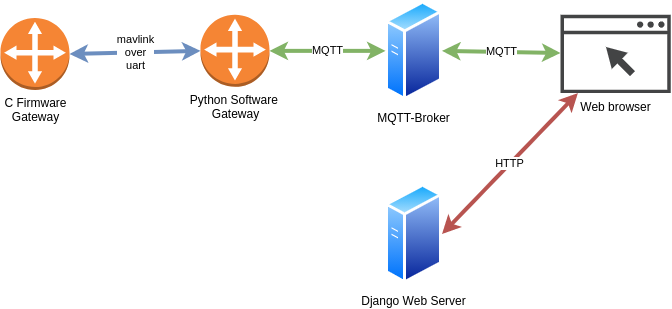
\includegraphics[scale=0.6]{software_architecture.png}
    \end{center}
    \caption{Software architecture}
    \label{fig:software_architecture}
\end{figure}

To make location related data available.

\section{UARTE}
The Universal asynchronous receiver/transmitter with EasyDMA (UARTE) offers fast, full-duplex, asynchronous serial communication with built-in flow control (CTS, RTS) support in hardware at a rate up to 1 Mbps, and EasyDMA data transfer from/to RAM.
\cite{nordic-semiconductor:nRF52832_PS_v1.4}

\section{MAVLink protocol}

\subsection*{What is MAVLink}
MAVLink is a very lightweight messaging protocol for communicating with drones (and between onboard drone components). \cite{web_mavlink}

\subsection*{MAVLink packet format}
\begin{figure}[H]
    \begin{center}
        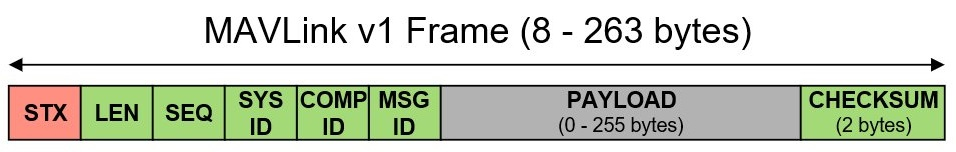
\includegraphics[scale=1.2]{packet_mavlink_v1.jpg}
    \end{center}
    \caption{MAVLink packet v1}
    \label{fig:packet_mavlink_v1}
\end{figure}

\subsection*{Pymavlink}

This is a Python implementation of the MAVLink protocol. It includes a source code generator (generator/mavgen.py) to create MAVLink protocol implementations for other programming languages as well. Also contains tools for analyzing flight logs.

\lstinputlisting[language=xml,
tabsize=3,
frame=lines,
caption=protocol.xml,
label=code:sample,
% frame=tlrb,
xleftmargin=20pt,
framexleftmargin=15pt,
keywordstyle=\color{blue}\bf,
commentstyle=\color{OliveGreen},
stringstyle=\color{red},
numbers=left,
numberstyle=\tiny,
numbersep=5pt,
breaklines=true,
showstringspaces=false,
basicstyle=\footnotesize,
emph={messages, enums},emphstyle={\color{magenta}}]{../../software/linux/gateway/protocol.xml}


\section{MQTT}
MQTT is an OASIS standard messaging protocol for the Internet of Things (IoT). It is designed as an extremely lightweight publish/subscribe messaging transport that is ideal for connecting remote devices with a small code footprint and minimal network bandwidth. MQTT today is used in a wide variety of industries, such as automotive, manufacturing, telecommunications, oil and gas, etc. \cite{web_mqtt_org}

\subsection*{Why MQTT?}

There are a number of reasons answering the question: Why MQTT is widely used in IOT? 
\begin{itemize}
    \item \textbf{Lightweight and efficient}: MQTT clients are very small, require minimal resources so can be used on small microcontrollers. MQTT message headers are small to optimize network bandwidth.
    \item \textbf{Bi-directional communications}: MQTT allows for messaging between device to cloud and cloud to device. This makes for easy broadcasting messages to groups of things.
    \item \textbf{Scale to millions of things}: MQTT can scale to connect with millions of IoT devices.
    \item \textbf{Reliable message delivery}: Reliability of message delivery is important for many IoT use cases. This is why MQTT has 3 defined quality of service levels: 0 - at most once, 1- at least once, 2 - exactly once
    \item \textbf{Support for unreliable networks}: Many IoT devices connect over unreliable cellular networks. MQTT’s support for persistent sessions reduces the time to reconnect the client with the broker.
    \item \textbf{Security enabled}: MQTT makes it easy to encrypt messages using TLS and authenticate clients using modern authentication protocols, such as OAuth.
\end{itemize}

\subsection*{MQTT publish/subscribe architecture}
\begin{figure}[H]
    \begin{center}
        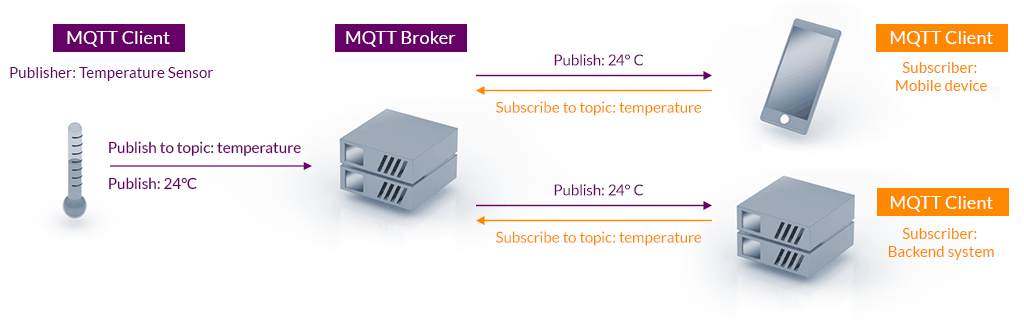
\includegraphics[scale=0.4]{mqtt-publish-subscribe.png}
    \end{center}
    \caption{MQTT publish subscribe}
    \label{fig:mqtt_publish_subscribe.}
\end{figure}

\subsection*{MQTT application message definition}

\section{Plotly}
Plotly JavaScript Open Source Graphing Library.

Built on top of d3.js and stack.gl, Plotly.js is a high-level, declarative charting library. plotly.js ships with over 40 chart types, including 3D charts, statistical graphs, and SVG maps.
plotly.js is free and open source and you can view the source, report issues or contribute on GitHub. \cite{web_plotly}

\subsection{Scatter plot}

\subsection{Circle plot}
\bib

\end{document}